%\clearpage
\section{6-3-5 Methode}\label{sec:635Methode}
Die 6-3-5 Methode ist eine Kreativitätstechnik zur Ideenfindung, optimalerweise wird Sie in einem Team mit 6 Personen angewendet. Es können Vorideen entstehen, wie auch gezielte Ideeanareicherung entwickelt werden.
\subsection{Vorgehensweise}
- In einem ersten Schritt werden Blätter in Papierform, jedem Teilenehmer verteilt, auf denen eine Tabelle mit 3 Spalten und die zuvor definierte Frage enthalten ist. Aus praktischen gründen sollten sich die Teilnehmer am selben Tisch befinden.\\
- Im zweiten Schritt sollte jeder Teilnehmer 3 Ideen zur Grundfrage, also meist eine Lösung für das definierte Problem, in je eine Spalte notieren. Die zeit zum nachdenken ist begrenzt auf 3 Minuten.\\
- In einem weiteren Schritt werden die Tabellen weitergegeben und die jeweils zuoberst beschriebenen Ideen können weiterentwickelt werden. Dieser Schritt wird im gesamten 5 mal durchgeführt.
\subsection{Vor- und Nachteile}
\begin{tabular}{|l|l|}
	\hline 
	Vorteile & Nachteile \\ 
	\hline 
	Jeder Teilnehmer kann seine Ideen & Keine Zeit für Fragen  \\
	 Notieren, keine dominanten Personen&\\ 
	\hline 
	Somit ist ein Protokoll erfasst&Es können Redundanzen entstehen \\ 
	\hline 
	Es entstehen in kurzer Zeit sehr viele&Arbeitstakt nicht für jeden Teilnehmer gleich\\
	interdisziplinäre Ideen&  \\ 
	\hline 
	Unnötige Diskussionen entfallen&Braucht eine Vorbereitung \\ 
	\hline 
	Jeder Teilnehmer muss sich beteiligen&  \\ 
	\hline 
\end{tabular} 
\subsection{Beispiel}
\begin{figure}[H]
	\centering
	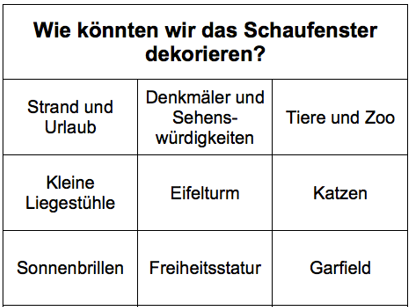
\includegraphics[width=0.5\textwidth]{M635.png}
	\caption{In dieser Abbildung kann erkannt werden, wie Ideen zur Frage: dekoration des Schafensters, entstanden sind}
	%\cite{thirah_vorhangeschloss-schlussel-computer-icons_nodate}
	%\raggedleft
\end{figure}
